%Settings for Bibliography Appendix
\renewcommand{\bibpreamble}{}
\renewcommand{\bibpostamble}{}
\renewcommand\bibfont{\normalfont\fontsize{8.58}{8}\selectfont}

%Content starts
\picturechapterlong{Curriculum vitae, List of publications, Acknowledgements}{Curriculum vitae, \\List of publications, \\Acknowledgements}{Chapter_covers/chapter_cover_7.pdf} \label{ch-7}
{
    \begin{center}
        \vspace*{4cm}
        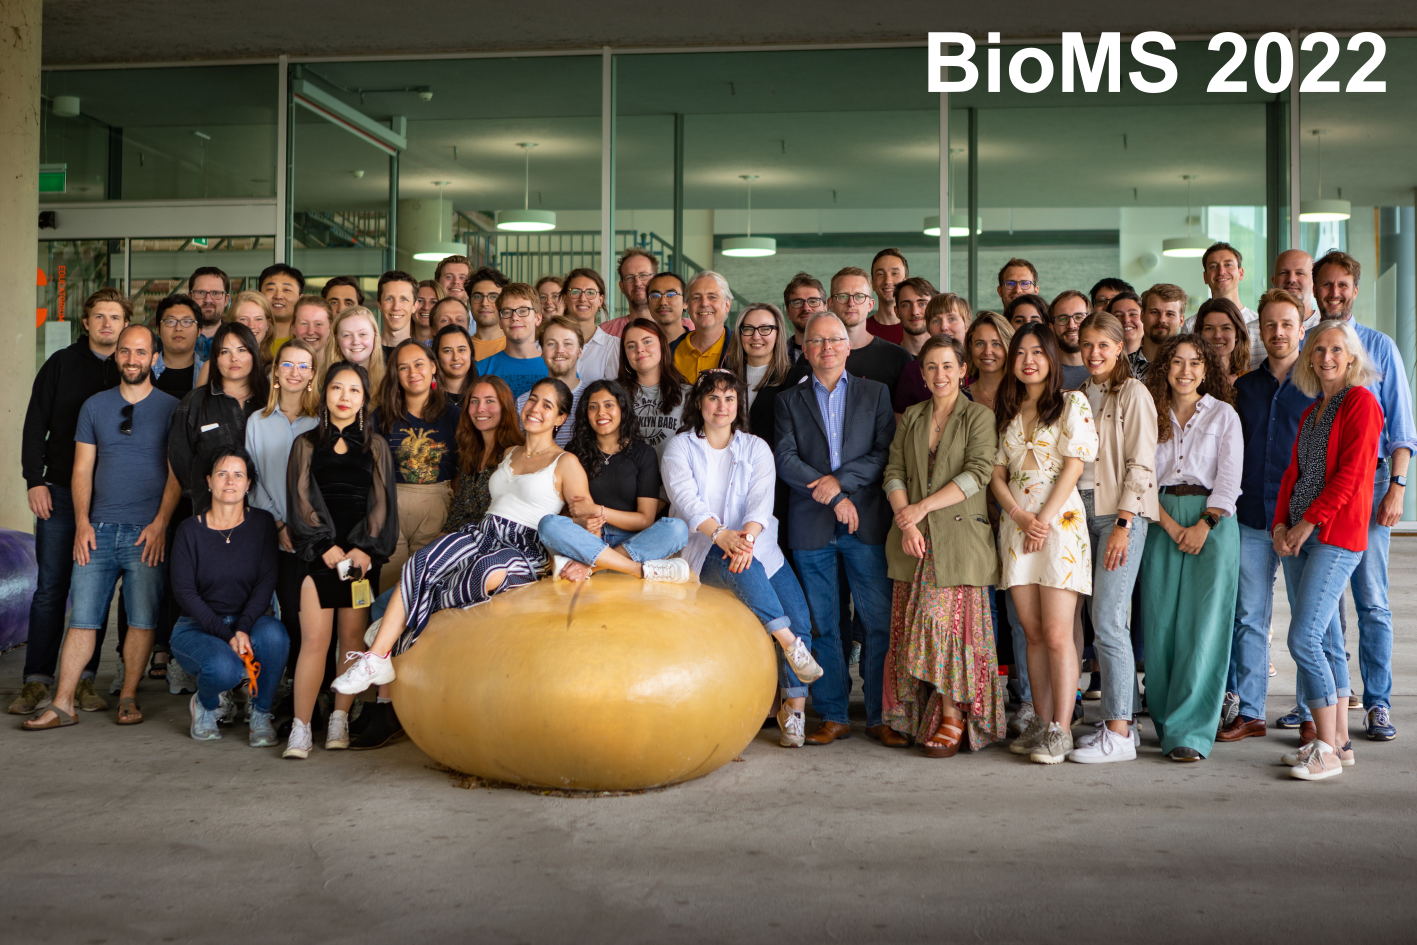
\includegraphics[]{Chapter.7/Figures/group_2022.png}
        \vspace{0.25cm}
    \end{center}
}
\clearpage
\section{Curriculum vitae}
I was born on the 12\textsuperscript{th} of December 1992 in Karlsruhe, Germany. After finishing high school in 2011, I worked and traveled before starting my Bachelor studies in Biotechnology in Berlin in 2013. During my studies I developed a strong interest in the structural characterization of proteins and protein complexes. The completion of my studies was marked by writing my Bachelor thesis entitled “\emph{Structural and functional analysis of spliceosomal Brr2-RNA-Helicase and its interaction partners}”, which I conducted in the research group of Prof. dr. Markus Wahl (Freie Universität Berlin). In 2016, I moved to Frankfurt am Main to pursue my Master studies, to further strengthen my structural biology toolshed. Amongst other research projects, I continued focusing on the structural characterization of protein and protein complexes using nuclear resonance microscopy (NMR) and X-ray crystallography within the group of Prof. dr. Wöhnert (Johann Wolfgang Goethe Universität, Frankfurt am Main). Realizing the importance of studying proteins and protein complexes in-vivo, I joined the research group of Dr. Mikhail Savitski (EMBL, Heidelberg) to conduct my Master thesis research entitled "\emph{Untangling the function of Escherichia coli genes by thermal proteome profiling (TPP)}". I applied mass spectrometry based techniques to shed further light on the function of a number of bacterial genes. Following my graduation in 2018, I moved to Utrecht, the Netherlands, and started a Ph.D. in the Biomolecular Mass Spectrometry group under the supervision of Prof. dr. Albert J.R. Heck in February 2019. Leveraging experiences gained in structural biology and mass spectrometry, we aimed at applying different structural proteomics techniques to structurally characterize novel proteins and protein complexes in mitochondria. Parts of the research performed during my PhD are presented in this thesis.
\clearpage
\section{List of publications}
\nocite{*}
\bibliographystyle{Style_settings/bibstyle_pnas}
\bibliography{Chapter.7/my_publications.bib}
\clearpage
\section{Acknowledgements}
When asking former PhD students about their PhD research experience, it is commonly described as “brutal, miserable, and life changing time”. I experienced my PhD research as truly exciting, miraculous, fun, and indeed life changing time that I will remember as one of the best things in my still (reasonably) young life. This positive experience is a result of extraordinary support and love that I received before, during (and hopefully after) my PhD, for which in the following lines, I would like to acknowledge the people who made all this possible.
I am deeply indebted to Albert. Thank you for the tangible and intangible support, your patience and most importantly for perfectly understanding how to handle, motivate and ameliorate me! I could not have asked for a better supervisor, and I will be forever grateful and hope that we will keep in close contact! On this note, I would also like to thank Misha and André. Without your guidance and support during my Master thesis project my PhD experience could never have been the same! You really prepared me to do a PhD and most importantly you were great role models in respect to the researcher I aspire to be!

Many thanks also to Riccardo, Pascal, and Barbara. You took me under your wing when I started my PhD and taught me everything you knew about mass spectrometers, liquid chromatography, cross-linking and computational modeling. Besides you are great friends with whom I had plenty of fun outside the lab, either playing soccer, running, having beers or dancing! I am extremely proud of what all of you have achieved and I am looking forward to visiting you in London, Grenoble, and Munich or wherever you are going to be! Likewise, special thanks to Richard, Andris, and Henk for the never-ending support you provided during these 4 years.

I was extremely lucky to have fruitful collaborations with experts outside of our lab, which resulted in publications forming a large part of this thesis. Dear Uli, Susanne and Alfredo thank you so much for the knowledge and expertise shared and all the additional support throughout my PhD. I am also thankful to Tzviya and Miguel. Working with you was nothing but amazing! I truly believe you do amazing science and I learned so much from you! Many thanks are also due to Nils, Dusanka and Jelena. I dearly enjoyed collaborating with you, not only did I gain new insights into the biology of the respiratory chain, but you also pushed me to further understand cross-linking data and to find new ways of analyzing it. It was a pleasure to work with you and I dearly hope that our efforts will be rewarded!

I further want to extend my sincere thanks to the Hecklab staff, without who the lab would not be functional and therefore equally responsible for my positive experience: Mirjam, Harm, Corine, Arjan, Ceri and Tatjana, thank you so much for always supporting, teaching, and helping me. I really appreciated working with you and I hope that I will have such uplifting, funny and amazing colleagues in the future.

Likewise, a big thank you is due to the entire Hecklab, every single person I met during my PhD was nothing but kind and supportive. I have amazing memories with all of you that I do not want to miss! Special thanks to Juan, Donna, Wouter, Danique, Gadi, Marteen and so many others, who always sweetened the lab parties and borrels for me. I will really miss our conversations as well as getting hydrated with you! Also special thanks to Julia: you are an amazing scientist and most importantly, a kind person and awesome friend! I will never forget your efforts aiming at making me the next Adam Ondra - sorry I failed so miserably. However, meeting you at the boulder gym and having a few or too many beers was always very enjoyable! Also dear thanks to Bastiaan: The moment we saw each other we knew it was going to be an ever-lasting friendship. Thank you so much for getting me started with bioinformatics but more importantly for being my first friend in the Netherlands! Thank you for making me feel home in Utrecht, either by inviting me to daylong BBQ adventures or nightlong game activities. I will truly miss not being able to see you daily. In addition, thanks to Douwe, my PhD latex adventure would have been not as “pleasant” as without you (I would not know whether I would have survived it). I also really like your enthusiasm about what you are doing and I am confident that you will have an amazing PhD!

Finally, I would like to thank important people “outside” the lab who supported me during this journey. Dear Tomislav, Sem and Voijta, you truly made the difference for me! Thank you for giving me valuable advice, always listening, accepting the beer pressure and simply for being amazing friends! You are great role models, and I am happy that you are in my life! Thank you for the weekly night outs and for enduring my high energy levels. I am always having a good time when I am with you! Likewise, I owe great gratitude to Clemont, Armin, Conor, Michelle, Valeria, and Sophia. Thank you so much for everything you have done for me, and your continuous support! I am extremely lucky to have you in my life and I will forever treasure our memories and cannot wait to make new once with you! Further, special thanks to my partner who not only endured me but who was and is a great source of support and love.
\begin{otherlanguage}{french}
    Morgane, merci beaucoup pour tout ton soutien, tes conseils et ton amour! Je suis si fier de toi et éternellement reconnaissant ! Merci mon bébé !
\end{otherlanguage}
And most importantly, In the last couple of lines I want to thank my family without whom I would have never accomplished anything. Special thanks to my mum and dad, grandparents and my brothers.
\begin{otherlanguage}{german}
    Mama, Papa, Oma, Opa, Sassa und Max, von ganzem Herzen danke ich euch für eure Unterstützung. Ihr seid das Wichtigste in meinem Leben und ich kann euch niemals genug danken für alles, was ihr für mich getan habt und tun werdet! Immer zusammen, niemals alleine!
\end{otherlanguage}



